%!TEX root = ../thesis.tex
\section{基本的な性能}
設計したロボットアームの基本的な性能を述べる.
\subsection{アームサイズ}
図\ref{fig:link_length}にロボットアームのアームリーチとリンク長を示す.人間の腕の長さの比\cite{humanarm:online}を参考に,肩から肘までは290㎜,肘から手首までは220㎜とした.アームリーチは660㎜であり,要求仕様の700㎜程度を満たしている.図\ref{fig:arm_size}にアームサイズを示す.比較のため,机とボトルを模したものを配置している.

\begin{figure}[htbp]
  \centering
  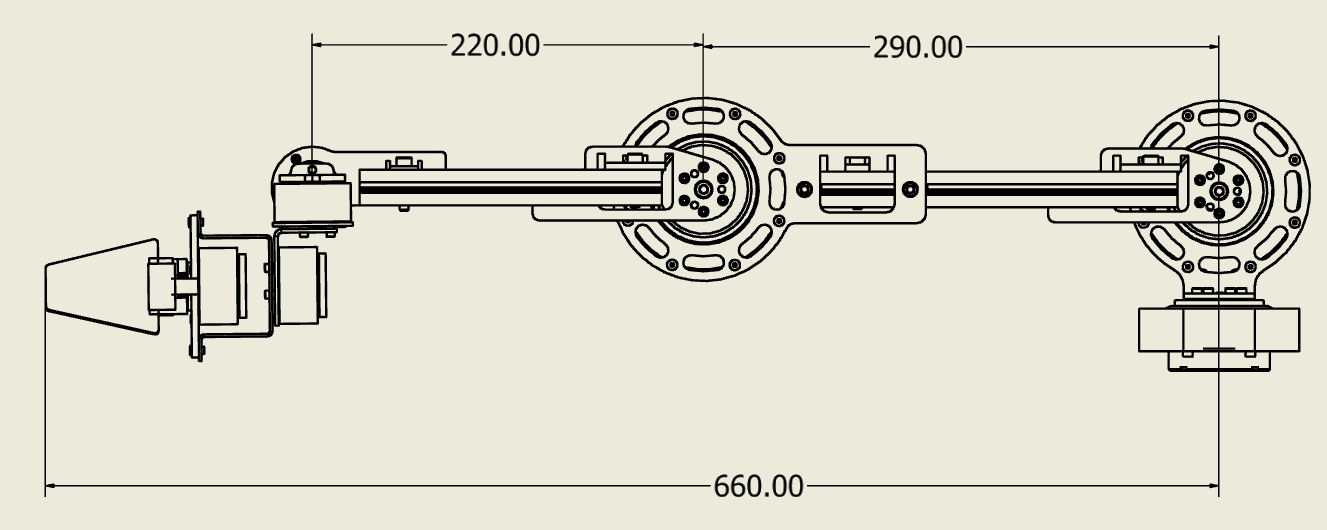
\includegraphics[width=10cm]{images/design/link_length.png}
  \caption{Arm reach and link length}
  \label{fig:link_length}
\end{figure}

\begin{figure}[htbp]
  \centering
  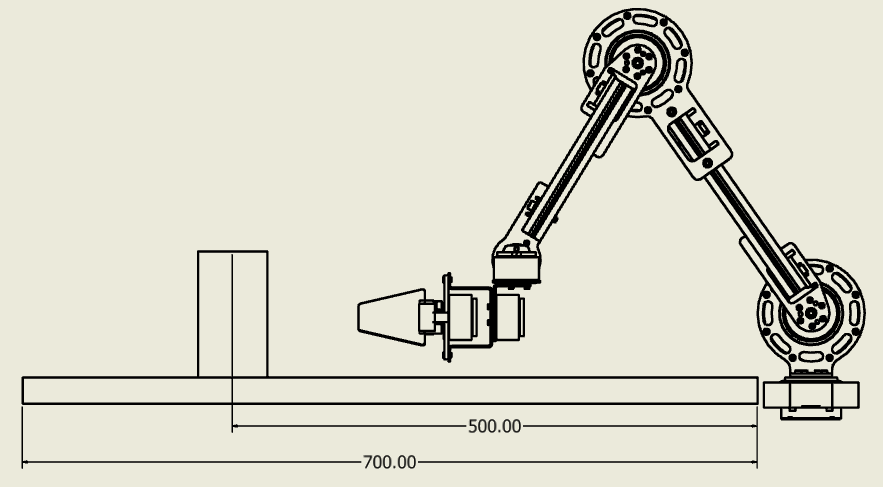
\includegraphics[width=10cm]{images/design/hikaku.png}
  \caption{Arm size}
  \label{fig:arm_size}
\end{figure}

\clearpage

\subsection{可動範囲}
図\ref{fig:arm_short},図\ref{fig:arm_long}にアームの最小可動範囲と最大可動範囲を示す.最小可動範囲は,アームの部品が干渉することなく動作できる最小の範囲を示しており,最大可動範囲はアームを最大まで伸ばしたときの範囲を示している.

\begin{figure}[htbp]
  \centering
  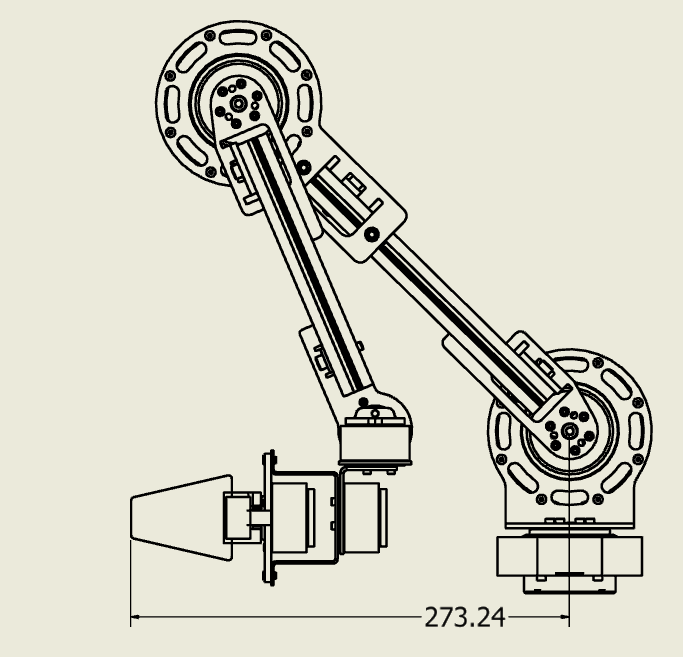
\includegraphics[width=10cm]{images/design/arm_short.png}
  \caption{Minimum range of motion}
  \label{fig:arm_short}
\end{figure}

\begin{figure}[htbp]
  \centering
  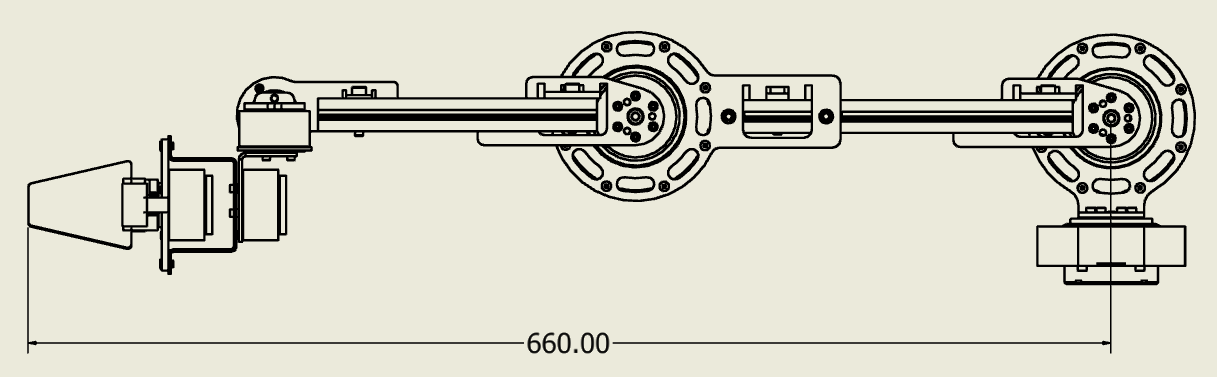
\includegraphics[width=10cm]{images/design/arm_long.png}
  \caption{Minimum range of motion}
  \label{fig:arm_long}
\end{figure}

\subsection{アームの手先の移動}
アームの手先の移動の様子を図\ref{fig:move1},図\ref{fig:move2},図\ref{fig:move3},図\ref{fig:move4}に示す.

\begin{figure}[h]
  \centering
  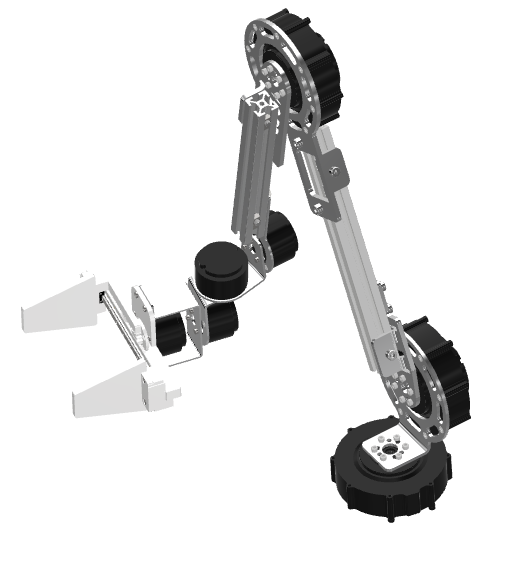
\includegraphics[width=10cm]{images/design/migitika.png}
  \caption{Stretched out to the right}
  \label{fig:move1}
\end{figure}

\begin{figure}[h]
  \centering
  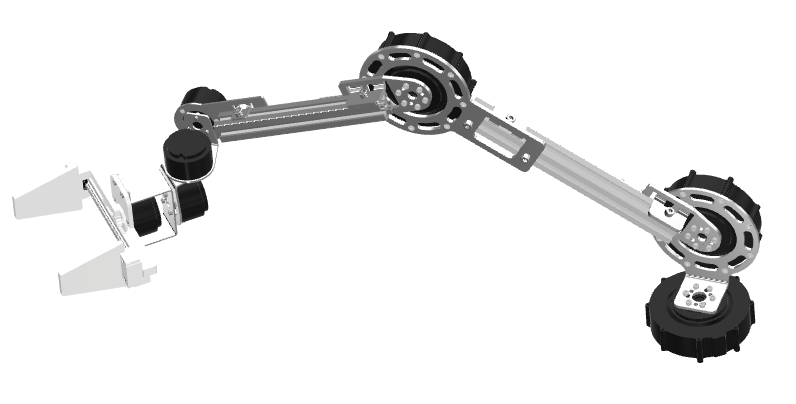
\includegraphics[width=10cm]{images/design/migioku.png}
  \caption{Stretched out to the right}
  \label{fig:move2}
\end{figure}

\begin{figure}[h]
  \centering
  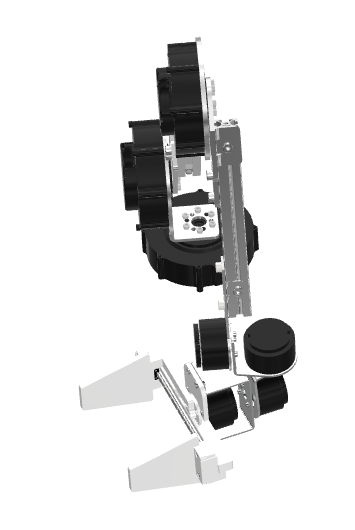
\includegraphics[width=8cm]{images/design/hidaritika.png}
  \caption{Stretched out to the left}
  \label{fig:move3}
\end{figure}

\begin{figure}[h]
  \centering
  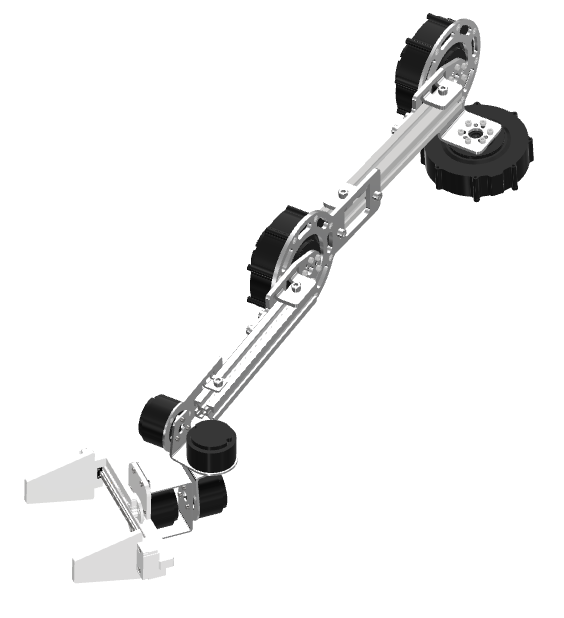
\includegraphics[width=10cm]{images/design/hidarioku.png}
  \caption{Stretched out to the left}
  \label{fig:move4}
\end{figure}
\clearpage

\subsection{可搬重量}
肩ピッチ軸のQDDモータ(SteadyWin GIM8108-8)の定格トルクは7.5Nm,最大トルクは22Nmである.アームを伸ばしたときに自重を支えるために必要なトルクを求め,常時把持することのできる物体の重量と,瞬間的に把持することのできる物体の重量を求める.
\subsubsection{自重を支える為に必要なトルク}
図\ref{fig:CoG}にアームの重心を示す.アームの重心は肩ピッチ軸から0.334mの位置にあり,アームの重さは1.31kgである.重力加速度を9.8m/s$^2$とすると,肩ピッチ軸にかかるトルク$T$は次のように求められる.
\begin{equation}
  T = 1.31 \times 9.8 \times 0.334 = 4.2 Nm
\end{equation}
\begin{figure}[h]
  \centering
  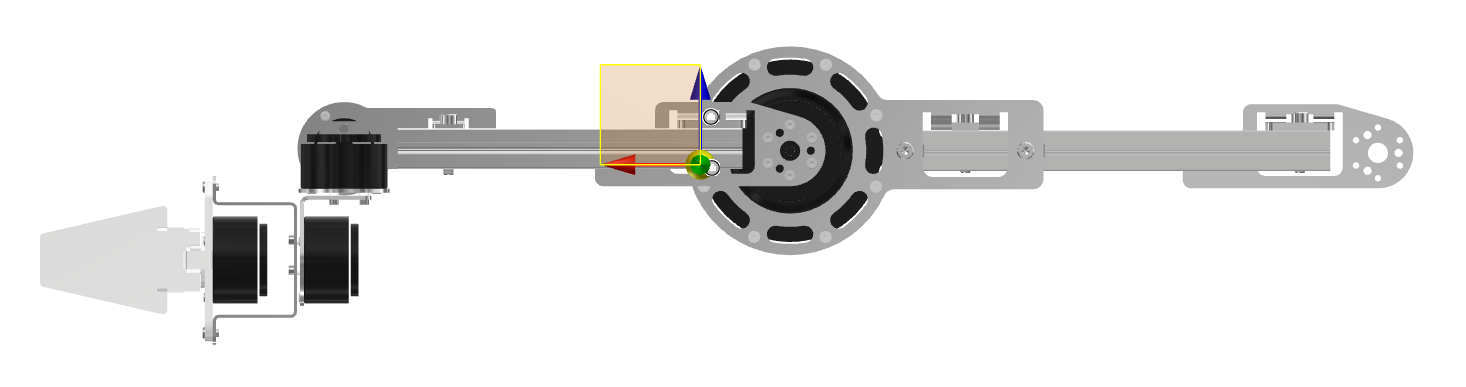
\includegraphics[width=10cm]{images/design/CoG.png}
  \caption{Center of gravity}
  \label{fig:CoG}
\end{figure}

\subsubsection{常時把持することのできる物体の重量}
アームの定格トルクから,自重を支える為に必要なトルクを引くと3.3Nmであり,肩ピッチ軸から手先までの距離は0.66mである.したがって,常時把持することのできる物体の重量$m$は次のように求められる.
\begin{equation}
  m = 3.3 / (9.8 \times 0.66) = 0.51kg
\end{equation}

\subsubsection{瞬間的に把持することのできる物体の重量}
同様に,最大トルクから自重を支える為に必要なトルクを引くと17.8Nmである.したがって,瞬間的に把持することのできる物体の重量$M$は次のように求められる.
\begin{equation}
  m = 17.8 / (9.8 \times 0.66) = 2.75kg
\end{equation}


\clearpage
\newpage